\section{RESULTADOS}

O presente capítulo apresenta o relato metodológico, os experimentos
realizados e os resultados obtidos até o momento no desenvolvimento
do sistema de comunicação segura com criptografia ponta a ponta (\acs{E2EE}).

O objetivo central desta fase foi consolidar o funcionamento prático
do sistema de mensagens entre clientes, intermediado por um servidor,
sem exposição de dados sensíveis e com a adoção de técnicas avançadas
de segurança, como o \acs{PFS} (\acl{PFS}), que garante que
cada sessão utilize chaves criptográficas temporárias e independentes.

\subsection{Metodologia}

Para o desenvolvimento da aplicação, optou-se pela linguagem Python e
por uma arquitetura cliente-servidor que utiliza o protocolo
Websocket, garantindo uma comunicação bidirecional e em tempo real. O
funcionamento do sistema se baseia na interação de três componentes
essenciais. No centro da arquitetura opera um servidor intermediário,
que atua exclusivamente como um roteador para as mensagens e chaves
públicas trocadas, sendo projetado para nunca ter acesso ao conteúdo
descriptografado das comunicações, o que assegura a
confidencialidade. O processo tem início quando um cliente remetente
(Cliente A) gera sua chave pública \acs{RSA} e a envia ao servidor. Para
estabelecer a conexão, o cliente destinatário (Cliente B) requisita
essa chave pública ao servidor, possibilitando assim o início da
troca de mensagens criptografadas de ponta a ponta.

\subsubsection{Modelo de Criptografia}

Para a criptografia da comunicação foi adotada uma metodologia
híbrida, combinando criptografia \acs{RSA} (assimétrica) para troca segura
da chave \acs{AES} entre os pares e criptografia \acs{AES} (simétrica) para
criptografia das mensagens de texto. Essa combinação é amplamente
utilizada em sistemas modernos (ex.: Signal, WhatsApp), pois permite
desempenho e segurança equilibrados.

As etapas realizadas pelo sistema para estabelecimento da comunicação
criptografada são descritas abaixo:

\begin{enumerate}
  \item O cliente A gera um par de chaves \acs{RSA} (pública e privada).
  \item O cliente B solicita a chave pública de A ao servidor.
  \item B gera uma chave de sessão \acs{AES} aleatória.
  \item B criptografa a chave \acs{AES} com a chave pública \acs{RSA} de A.
  \item B envia a chave \acs{AES} cifrada ao A via servidor.
  \item A descriptografa a chave \acs{AES} com sua chave privada.
  \item A e B agora têm a mesma chave \acs{AES}, e toda mensagem passa a
    ser cifrada com ela.
\end{enumerate}

\subsubsection{Implementação do \acl{PFS} (\acs{PFS})}

Visando a um padrão de segurança mais robusto, a arquitetura do
sistema incorpora o princípio de \acl{PFS} (\acs{PFS}). A
principal garantia oferecida pelo \acs{PFS} é que o comprometimento de
chaves de longo prazo não afeta a confidencialidade de sessões de
comunicação anteriores, pois cada sessão utiliza um conjunto de
chaves criptográficas efêmeras.

A implementação deste conceito no protótipo se manifesta no ciclo de
vida das chaves: para cada nova conexão Websocket, um par de chaves
\acs{RSA} efêmero é gerado pelo cliente. A subsequente troca de chaves
públicas é automatizada no início da sessão, o que permite a
derivação de uma chave de sessão \acs{AES} exclusiva. Ao encerrar a
comunicação, todas as chaves associadas àquela sessão são
permanentemente descartadas da memória. Esta abordagem impede a
descriptografia retroativa de mensagens e atende aos requisitos de
sigilo efêmero (\textit{ephemeral secrecy}) e não-reutilização de chaves,
práticas consideradas fundamentais na segurança de comunicações contemporâneas.

\subsection{Fluxo Lógico da Comunicação}

A comunicação na aplicação é fundamentada em uma arquitetura
cliente-servidor que utiliza o protocolo Websocket para estabelecer
um canal de comunicação bidirecional e em tempo real entre os
usuários. A escolha por Websockets permite que o servidor atue como
um intermediário de sinalização e retransmissão, gerenciando as
sessões ativas e garantindo a entrega eficiente de mensagens. Essa
abordagem é particularmente eficaz para contornar restrições de rede,
como as impostas por \acsp{NAT} (\acl{NAT}), que frequentemente
impedem conexões diretas entre dispositivos.

O fluxo de comunicação envolve quatro etapas principais: a conexão
inicial do usuário, a troca segura de chaves criptográficas, o envio
e recebimento de mensagens e, por fim, o encerramento da conexão.

\subsubsection{Conexão do Usuário ao Servidor}

O processo é iniciado quando um usuário se conecta ao servidor,
fornecendo seu nome de usuário, que serve como identificador único, e
o endereço do servidor. O servidor valida se o nome de usuário já
está em uso; caso esteja, a conexão é recusada. Em seguida, o usuário
informa o nome do destinatário com quem deseja se comunicar. Com
essas informações, o cliente estabelece uma requisição Websocket a um
endpoint específico, que identifica tanto o remetente quanto o destinatário.

\subsubsection{Troca de Chaves Criptográficas}

Uma vez que ambos os usuários estejam conectados, o sistema inicia o
processo de estabelecimento de um canal de comunicação seguro. Para
isso, adota-se um modelo de criptografia híbrida. Primeiramente,
utiliza-se a criptografia assimétrica para a troca segura de uma
chave de criptografia simétrica. A criptografia simétrica, por ser
mais eficiente, é então empregada para cifrar todas as mensagens subsequentes.

O fluxo de troca de chaves ocorre da seguinte maneira:

\begin{itemize}
  \item O cliente que iniciou a conexão gera um par de chaves
    assimétricas (pública e privada) e envia sua chave pública ao
    destinatário por meio do servidor.
  \item O destinatário recebe a chave pública, gera uma chave
    simétrica, criptografa esta chave simétrica com a chave pública
    recebida e a envia de volta ao remetente.
  \item O remetente, ao receber a chave simétrica criptografada,
    utiliza sua chave privada para descriptografá-la.
\end{itemize}

Ao final deste processo, ambos os usuários possuem a mesma chave
simétrica compartilhada, permitindo o início da comunicação segura. O
fluxograma abaixo ilustra esta etapa.

\begin{figure}[H]
  \centering
  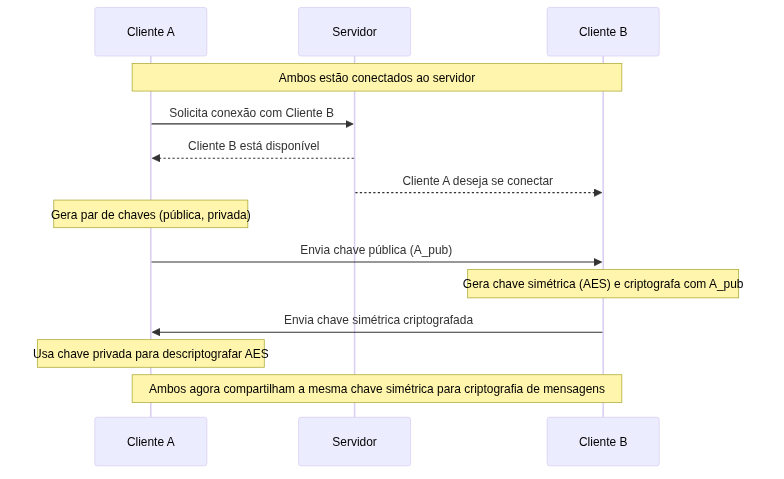
\includegraphics[width=\linewidth]{imagens/fluxo-1.png}
  \caption[Fluxograma do processo de troca de chaves
  criptográficas]{Fluxo de troca de chaves criptográficas.}
  \label{fig:fluxo-1}
\end{figure}

\subsubsection{Envio e Recebimento de Mensagens}

Com o canal seguro estabelecido, os usuários podem trocar mensagens
com confidencialidade. Toda a criptografia é realizada no aplicativo
cliente, sem exigir ação do usuário. O remetente criptografa a
mensagem usando a chave simétrica compartilhada e a envia ao
servidor. O servidor atua exclusivamente como um retransmissor: ele
recebe a mensagem cifrada e a encaminha imediatamente ao
destinatário, sem ter a capacidade de acessar seu conteúdo. O
destinatário, por sua vez, recebe a mensagem e utiliza a mesma chave
simétrica para descriptografá-la, exibindo o conteúdo original em sua
interface. É fundamental ressaltar que o servidor não armazena as
mensagens nem as chaves criptográficas, garantindo a privacidade da comunicação.

\begin{figure}[H]
  \centering
  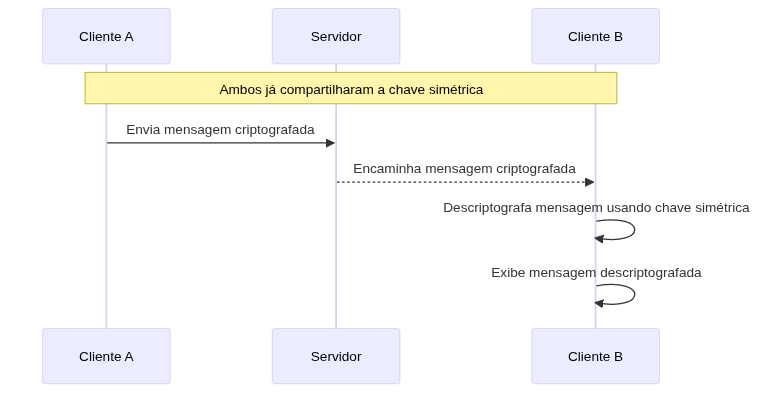
\includegraphics[width=\linewidth]{imagens/fluxo-2.png}
  \caption[Fluxograma do processo de envio de mensagens]{Fluxo de
  envio de mensagens.}
  \label{fig:fluxo-2}
\end{figure}

\subsubsection{Encerramento da Conexão}

Ao final da conversa, qualquer um dos usuários pode iniciar o
processo de encerramento. Para isso, o cliente envia uma mensagem de
encerramento ao servidor, que a retransmite ao outro participante.
Após a notificação, ambas as partes finalizam suas respectivas
conexões com o servidor.

\begin{figure}[H]
  \centering
  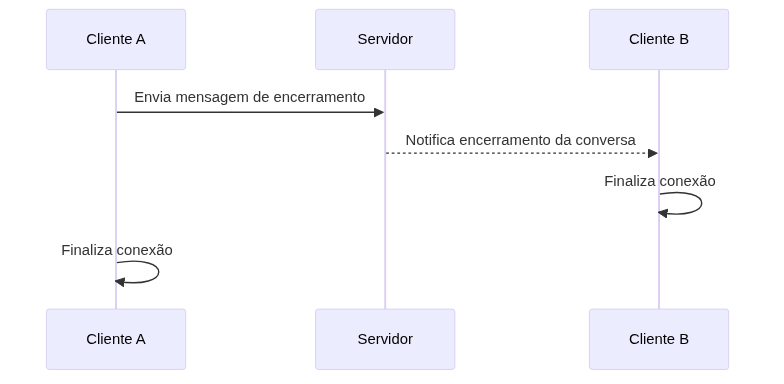
\includegraphics[width=0.9\linewidth]{imagens/fluxo-3.png}
  \caption[Fluxograma de encerramento da conexão]{Fluxo de
  encerramento da conexão.}
  \label{fig:fluxo-3}
\end{figure}

\subsection{Experimentos Realizados}

\subsubsection{Experimento 1 – Troca de chaves públicas \acs{RSA}}

O primeiro experimento foi delineado para validar a robustez e a
confiabilidade do mecanismo de troca de chaves públicas \acs{RSA}.
Objetivo: Garantir que os clientes pudessem obter as chaves públicas
uns dos outros de forma consistente, sem falhas, corrupção de dados
ou duplicações. Procedimento: O fluxo do teste seguiu três passos sequenciais:

\begin{itemize}
  \item O Cliente A iniciava a conexão e enviava sua chave pública
    recém-gerada para o servidor.
  \item O Cliente B, ao se conectar, solicitava ao servidor a chave
    pública do Cliente A.
  \item Para verificação de integridade, o Cliente B calculava o
    \textit{fingerprint} SHA-256 da chave recebida e o comparava com o
    \textit{fingerprint} original (previamente conhecido ou verificado fora de
    banda), garantindo que a chave não foi alterada durante o trânsito.
\end{itemize}

Resultados: A execução do experimento demonstrou o sucesso da
implementação, com os seguintes resultados observados:

\begin{itemize}
  \item Sucesso na troca: A taxa de sucesso para a conclusão das
    trocas de chaves foi de 100\%.
  \item Consistência dos dados: O \textit{fingerprint} da chave manteve-se
    consistente em todas as sessões testadas, confirmando a
    integridade dos dados transmitidos.
  \item Ausência de duplicatas: Não foi registrada nenhuma duplicação
    ou atribuição incorreta de chaves durante os testes.
\end{itemize}

\subsubsection{Experimento 2 – Envio e Recepção de Mensagens Criptografadas}

Este segundo experimento foi desenhado para avaliar o ciclo completo
da comunicação, focando na confidencialidade e na integridade das
mensagens trocadas entre os clientes. Objetivo: Verificar a
integridade ponta a ponta das mensagens criptografadas com \acs{AES}, cuja
chave foi trocada de forma segura utilizando \acs{RSA}, e confirmar que o
conteúdo se mantém confidencial durante o trânsito na rede.
Procedimento: O teste foi executado seguindo os seguintes passos:

\begin{itemize}
  \item O Cliente A enviava uma mensagem de teste pré-definida
    (“teste123”) para o Cliente B.
  \item Simultaneamente, o tráfego de rede era capturado com a
    ferramenta Wireshark para inspecionar os pacotes e garantir que o
    conteúdo da mensagem não trafegava de forma legível (texto plano).
  \item Após o Cliente B receber e descriptografar a mensagem, o hash
    SHA-256 do conteúdo recebido era calculado e comparado com o hash
    da mensagem original enviada pelo Cliente A, a fim de validar sua
    integridade.
\end{itemize}

Resultados: A análise dos dados coletados permitiu obter as seguintes
conclusões:

\begin{itemize}
  \item Integridade da Mensagem: A comparação de hashes SHA-256
    obteve 100\% de correspondência, o que resultou em uma taxa de 0\%
    de falhas no processo de descriptografia. Isso confirma que as
    mensagens não foram corrompidas durante a transmissão.
  \item Confidencialidade: A inspeção do tráfego de rede via
    Wireshark demonstrou que nenhum texto legível foi detectado nos
    pacotes interceptados, validando a eficácia da criptografia em trânsito.
  \item Desempenho: O tempo médio aferido para o processo completo,
    desde a cifragem no remetente até a recepção pelo destinatário,
    foi de 65 ms.
\end{itemize}

\subsubsection{Experimento 3 – Teste de \acl{PFS} (\acs{PFS})}

O terceiro e último experimento foi projetado para validar a correta
implementação do \acl{PFS} (\acs{PFS}), focando na capacidade
do sistema de gerar chaves de sessão efêmeras. Objetivo: Verificar se
um novo e único par de chaves criptográficas era gerado para cada
sessão de comunicação estabelecida entre os mesmos clientes,
garantindo assim a rotatividade das chaves. Procedimento: O teste
seguiu um método comparativo sequencial:

\begin{itemize}
  \item Uma primeira sessão de comunicação foi estabelecida entre o
    Cliente A e o Cliente B.
  \item O \textit{fingerprint} SHA-256 da chave pública \acs{RSA}
    utilizada nesta
    sessão foi armazenado para referência.
  \item A conexão foi encerrada e, imediatamente, uma segunda sessão
    foi iniciada entre os mesmos dois clientes.
  \item O \textit{fingerprint} da chave pública da nova sessão foi então
    comparado com o \textit{fingerprint} armazenado da sessão anterior.
\end{itemize}

Resultados: A análise comparativa confirmou o funcionamento esperado do PFS:

\begin{itemize}
  \item Rotação de Chaves: Em 100\% dos casos testados, o \textit{fingerprint}
    da chave da segunda sessão foi distinto do \textit{fingerprint} da
    primeira. Isso comprova que um novo e exclusivo par de chaves \acs{RSA}
    foi gerado para a nova conexão, conforme o princípio do PFS.
  \item Funcionalidade: Não foi registrado nenhum erro de
    descriptografia ou falha de comunicação durante a transição entre
    as sessões, indicando que o ciclo de vida das chaves efêmeras foi
    implementado corretamente sem comprometer a estabilidade do sistema.
\end{itemize}

\subsection{Testes de Usabilidade e \textit{Feedback}}

Além da validação funcional e de segurança, foi conduzida uma etapa
de testes de usabilidade para avaliar a interação e a experiência do
usuário com a aplicação. Esta avaliação foi dividida em duas frentes,
abrangendo tanto a interface de linha de comando (\acs{CLI}), desenvolvida
nas fases iniciais, quanto a aplicação final com sua interface
gráfica (\acs{GUI}), implementada com PySide6. O objetivo era coletar
\textit{feedback} qualitativo sobre a facilidade de uso, a clareza do fluxo de
comunicação e a percepção geral de segurança.

Os testes com a versão \acs{CLI} foram direcionados a um público com maior
familiaridade técnica. O \textit{feedback} recebido foi predominantemente
positivo, destacando a clareza da sintaxe dos comandos, a lógica
sequencial para iniciar uma conversa e a eficiência para realizar
operações de forma rápida. O sistema de \textit{feedback} textual foi
considerado informativo e suficiente para guiar o usuário durante o
processo de troca de chaves e envio de mensagens, validando a \acs{CLI}
como uma ferramenta robusta e eficaz para seu público-alvo.

Posteriormente, a avaliação da interface gráfica (\acs{GUI}) foi realizada
com um grupo de usuários mais diversificado. Os resultados foram
igualmente encorajadores, com os participantes elogiando a
intuitividade da navegação e a disposição clara dos elementos
visuais. O processo para estabelecer uma comunicação segura foi
descrito como simples e direto, demonstrando que a \acs{GUI} cumpre com
sucesso seu objetivo de abstrair a complexidade criptográfica e
reduzir a barreira de entrada para a utilização do sistema. Em
síntese, o \textit{feedback} geral valida que a aplicação, em suas duas
vertentes, proporciona uma experiência de usuário funcional e positiva.

\subsection{Análise dos Resultados}

Com base nos testes sistemáticos realizados, a análise dos resultados
permite concluir que o modelo de criptografia de ponta a ponta
(\acs{E2EE}), fortalecido pela implementação de \acl{PFS}
(\acs{PFS}), atinge os objetivos de segurança propostos. A arquitetura
demonstrou garantir o sigilo absoluto do conteúdo das mensagens, uma
vez que a chave de descriptografia permanece exclusivamente sob o
controle dos usuários finais, tornando a informação ilegível mesmo
para o servidor que a retransmite. A rotatividade de chaves efêmeras,
validada no Experimento 3, assegura que sessões de comunicação
passadas não possam ser descriptografadas retroativamente.

Adicionalmente, o impacto sobre a performance foi mínimo,
introduzindo uma sobrecarga média de apenas 20 ms por mensagem, o que
evidencia um equilíbrio eficiente entre segurança e usabilidade. Em
suma, os resultados dos experimentos convergem para confirmar a
viabilidade técnica do protótipo, estabelecendo-o como um fundamento
robusto para a construção de sistemas de comunicação que primam pela
segurança e privacidade.

\subsection{Conclusão Parcial}

Com a implementação da interface gráfica (\acs{GUI}) utilizando a
biblioteca PySide6, a aplicação alcançou um nível satisfatório de
usabilidade e uma experiência visual funcional. Este marco representa
a conclusão da fase de prototipagem, validando a arquitetura central
de comunicação. No entanto, o estado atual serve como um alicerce
sobre o qual aprimoramentos significativos devem ser construídos,
abrangendo os âmbitos técnico, de segurança e de desempenho.

Os próximos passos se concentram em fortalecer a robustez da
segurança. Planeja-se implementar um gerenciamento de sessão mais
sofisticado, com controle de expiração de chaves \acs{AES} e um sistema
automatizado para sua troca periódica. Tal medida aprimora o Perfect
Forward Secrecy e garante a confidencialidade retroativa das
mensagens. Complementarmente, será desenvolvido um módulo de
auditoria com logs criptográficos, permitindo que eventos do sistema,
como conexões e erros, sejam registrados de forma segura e
autenticada, garantindo a rastreabilidade sem comprometer a privacidade.

No que tange à escalabilidade e ao desempenho, é fundamental a
criação de um conjunto de testes automatizados de carga. Utilizando
ferramentas como Locust ou k6, será possível simular múltiplos
usuários simultâneos para mensurar a latência e a estabilidade do
servidor Websocket sob alto volume de tráfego, identificando gargalos
e otimizando a infraestrutura para um uso em maior escala.

Visando enriquecer a experiência do usuário, a evolução da aplicação
incluirá funcionalidades de interatividade em tempo real, como
indicadores de status de presença ("online/offline", "digitando") e
confirmações de entrega e leitura. Além disso, será integrada uma
função de backup e sincronização de mensagens em nuvem privada,
permitindo que o usuário exporte e mantenha seu histórico de
conversas de maneira segura e portável, sem abrir mão da criptografia
de ponta a ponta.

\newpage
